%%%%%%%%%%%%%%%%%%%%%%%%%%%%%%%%%%%%%%%%%%%%%%%%%%%%%%%%%%%%%%%%%%%%
%% UNSW SENG2020 2012S2 GROUP 6 REPORT TEMPLATE
%% CREATED BY VINCENT WONG
%%%%%%%%%%%%%%%%%%%%%%%%%%%%%%%%%%%%%%%%%%%%%%%%%%%%%%%%%%%%%%%%%%%%

\documentclass[a4paper]{article}
\usepackage{a4wide}
\usepackage{longtable}
\usepackage[normalem]{ulem}     %% gives strikeout capability with \sout{}
\usepackage{graphicx}
\usepackage{float}
\usepackage[usenames,dvipsnames]{color}
\RequirePackage{bsymb,b2latex}
%%%%%%%%%%%%%%%%%%%%%%%%%%%%%%%%%%%%%%%%%%%%%%%%%%%%%%%%%%%%%%%%%%%%%
%% DOCUMENT MACROS -- DO NOT DELETE


\begin{document}

%%%%%%%%%%%%%%%%%%%%%%%%%%%%%%%%%%%%%%%%%%%%%%%%%%%%%%%%%%%%%%%%%%%%%
%% TITLE PAGE
\thispagestyle{empty}      % turn off page numbering
\begin{center}
\Large\textbf{$\odot\int$ Sale} %%\odot \int Sale

\Large\textbf{Design Report}

%%%% MAKE SURE YOU SPECIFY YOUR GROUP NUMBER
\bigskip\large\textbf{Group Number: 06}
\end{center}

\vspace*{16.5cm}
\begin{tabular}{|l|l|}
  \hline
  Version         & 1.0\\\hline
  Print Date      & 15/09/2012 13:37\\\hline
  Release Date    & 15/09/2012\\\hline
  Release State   & Final\\\hline
  Approval State  & Pending\\\hline
  Approved by     & Chris, Dylan, Lasath, Vincent\\\hline
  Prepared by     & Chris, Dylan, Lasath, Vincent\\\hline
  Reviewed by     & Chris, Dylan, Lasath, Vincent\\\hline
  Confidentiality Category  & Public\\\hline
\end{tabular}
\pagebreak

%%%%%%%%%%%%%%%%%%%%%%%%%%%%%%%%%%%%%%%%%%%%%%%%%%%%%%%%%%%%%%%%%%%%%
%% REVISION CONTROL PAGE
\thispagestyle{plain}     % Turn on page numbering
\setcounter{page}{1}      % set page number counter
\renewcommand{\thepage}{\roman{page}}  % set page number to roman

\noindent{\Large\textbf{Document Revision Control}}\\[2ex]
\begin{tabular}{|l|l|l|l|}
  \hline
  Version & Date & Authors & Summary of Changes\\\hline\hline
  0.1 & 03/08/2012     &    Vincent     &    Created initial report               \\\hline
   0.2 & 03/08/2012     &    Lasath     &    Added Architecture section               \\\hline
 
\end{tabular}

\pagebreak

%%%%%%%%%%%%%%%%%%%%%%%%%%%%%%%%%%%%%%%%%%%%%%%%%%%%%%%%%%%%%%%%%%%%%
%% TABLE OF CONTENTS AND FIGURES

\tableofcontents
\pagebreak


%%%%%%%%%%%%%%%%%%%%%%%%%%%%%%%%%%%%%%%%%%%%%%%%%%%%%%%%%%%%%%%%%%%%%
%% MAIN DOCUMENT
\setcounter{page}{1}     % Set page number counter
\renewcommand{\thepage}{\arabic{page}}  % print page number as arabic

%%%%%%%%%%%%%%  THIS IS WHERE YOU PUT YOUR CONTENT %%%%%%%%%%%%%%%%%%

\section{Overview and Design Considerations}

The Point of Sale/Warehouse System (PosWare) is designed to be a simple yet sophisticated system which provides extensive sales and logistics management functionality to all kinds of businesses from large to small. 

Our system has to be able to be deployed across multiple machines to suit the needs of medium to large businesses. This allows for cashiers and stock controllers to be in separate locations while working on the same system and also allows multiple cashiers to be active at once (as stated by requirement DN {{@requirement_id}}. However this does contrast to the capabilities of EventB, which models a single system with a state and purely atomic operations and would be difficult to implement whilst spread over multiple machines. 

In an attempt to stick as close to the model as possible, we decided to store all state in a database. Since all machines can access this database it essentially allows for a single shared state between the machines.

Events were converted into methods (as explained in detail in section {@balh}), which will run in a central server. Since all state is maintained within the database, it is unnecessary for these methods/classes to maintain any local state. If fact, doing so is likely to cause unintended consequences or extra side effects. In order to keep these methods atomic, to match model events, they were restricted to one database update query per method (except during rare special circumstances) .

Keeping the methods in classes which maintain no state on themselves during execution, whilst allowing us to match the model events, also caused another advantage; they can be executed on different machines. This will allow for good scalability in case of large businesses with lots of machines, they can merely have multiple of servers with distributed load balancing. 

This leaves most of the machines as thin clients since they will only need to perform enquiry services rather than individual processing. At this time we are considering making these clients web based for the ease of deployment. 

The system will have a backup servers in case issues arise from the system in-store. All the data will be backed up offsite on the user’s choice of cloud storage provider. The system will be made such that if any issues arise with the onsite servers, requests can be redirected to offsite servers temporarily while the issue gets resolved.The terminals can be replaced if broken as our system has no reliance on the terminal for the system functionality. 

We will have 3 key types of user interfaces in this system and each will run on thin clients. These include the Cashiers UI which will be run on the cash registers, Stock controller UI which will be run on backroom machines, and the manager UI which can be run anywhere throughout the system. 



\pagebreak

\section{Class Overview }

Our system is split up into 10 main classes that are core to the design of the system. There are a number of atomic classes that are crucial to the functionality of the point of sales system. Such classes include products, locations, users, sales, and transactions. These classes were evident in both our requirements and our event-b model. The product class has many relations, one of which is a product’s quantity in a stock location. The product class is also linked to suppliers, orders, sales.

As described in our requirements it has one major link, which is that of the products thresholds and levels. The other is through that of stockorders between the locations. The next two key class to our system is that of suppliers and supplier stock orders these are both related to the product and are the events which allow for our system to meet the requirements which allowed for automatic ordering two suppliers.  

The rest of our classes are mainly those involved with the sales of items and there payments. A sale allows ust o have many sale-items, aswell as multiple payments and also a customer and a worker. These combined allow us to meed all the requirements, within our system by directly relating to your event-b.

The workers and the customers in the system are represented as users, and all the attributes provide the features that were required by our system. It allowed us to create and edit the users as well as apply discounts for both staff and custmers, as described by our requirements system. 

\pagebreak
\section{Class Diagram}

\begin{figure}[h]
\centering
  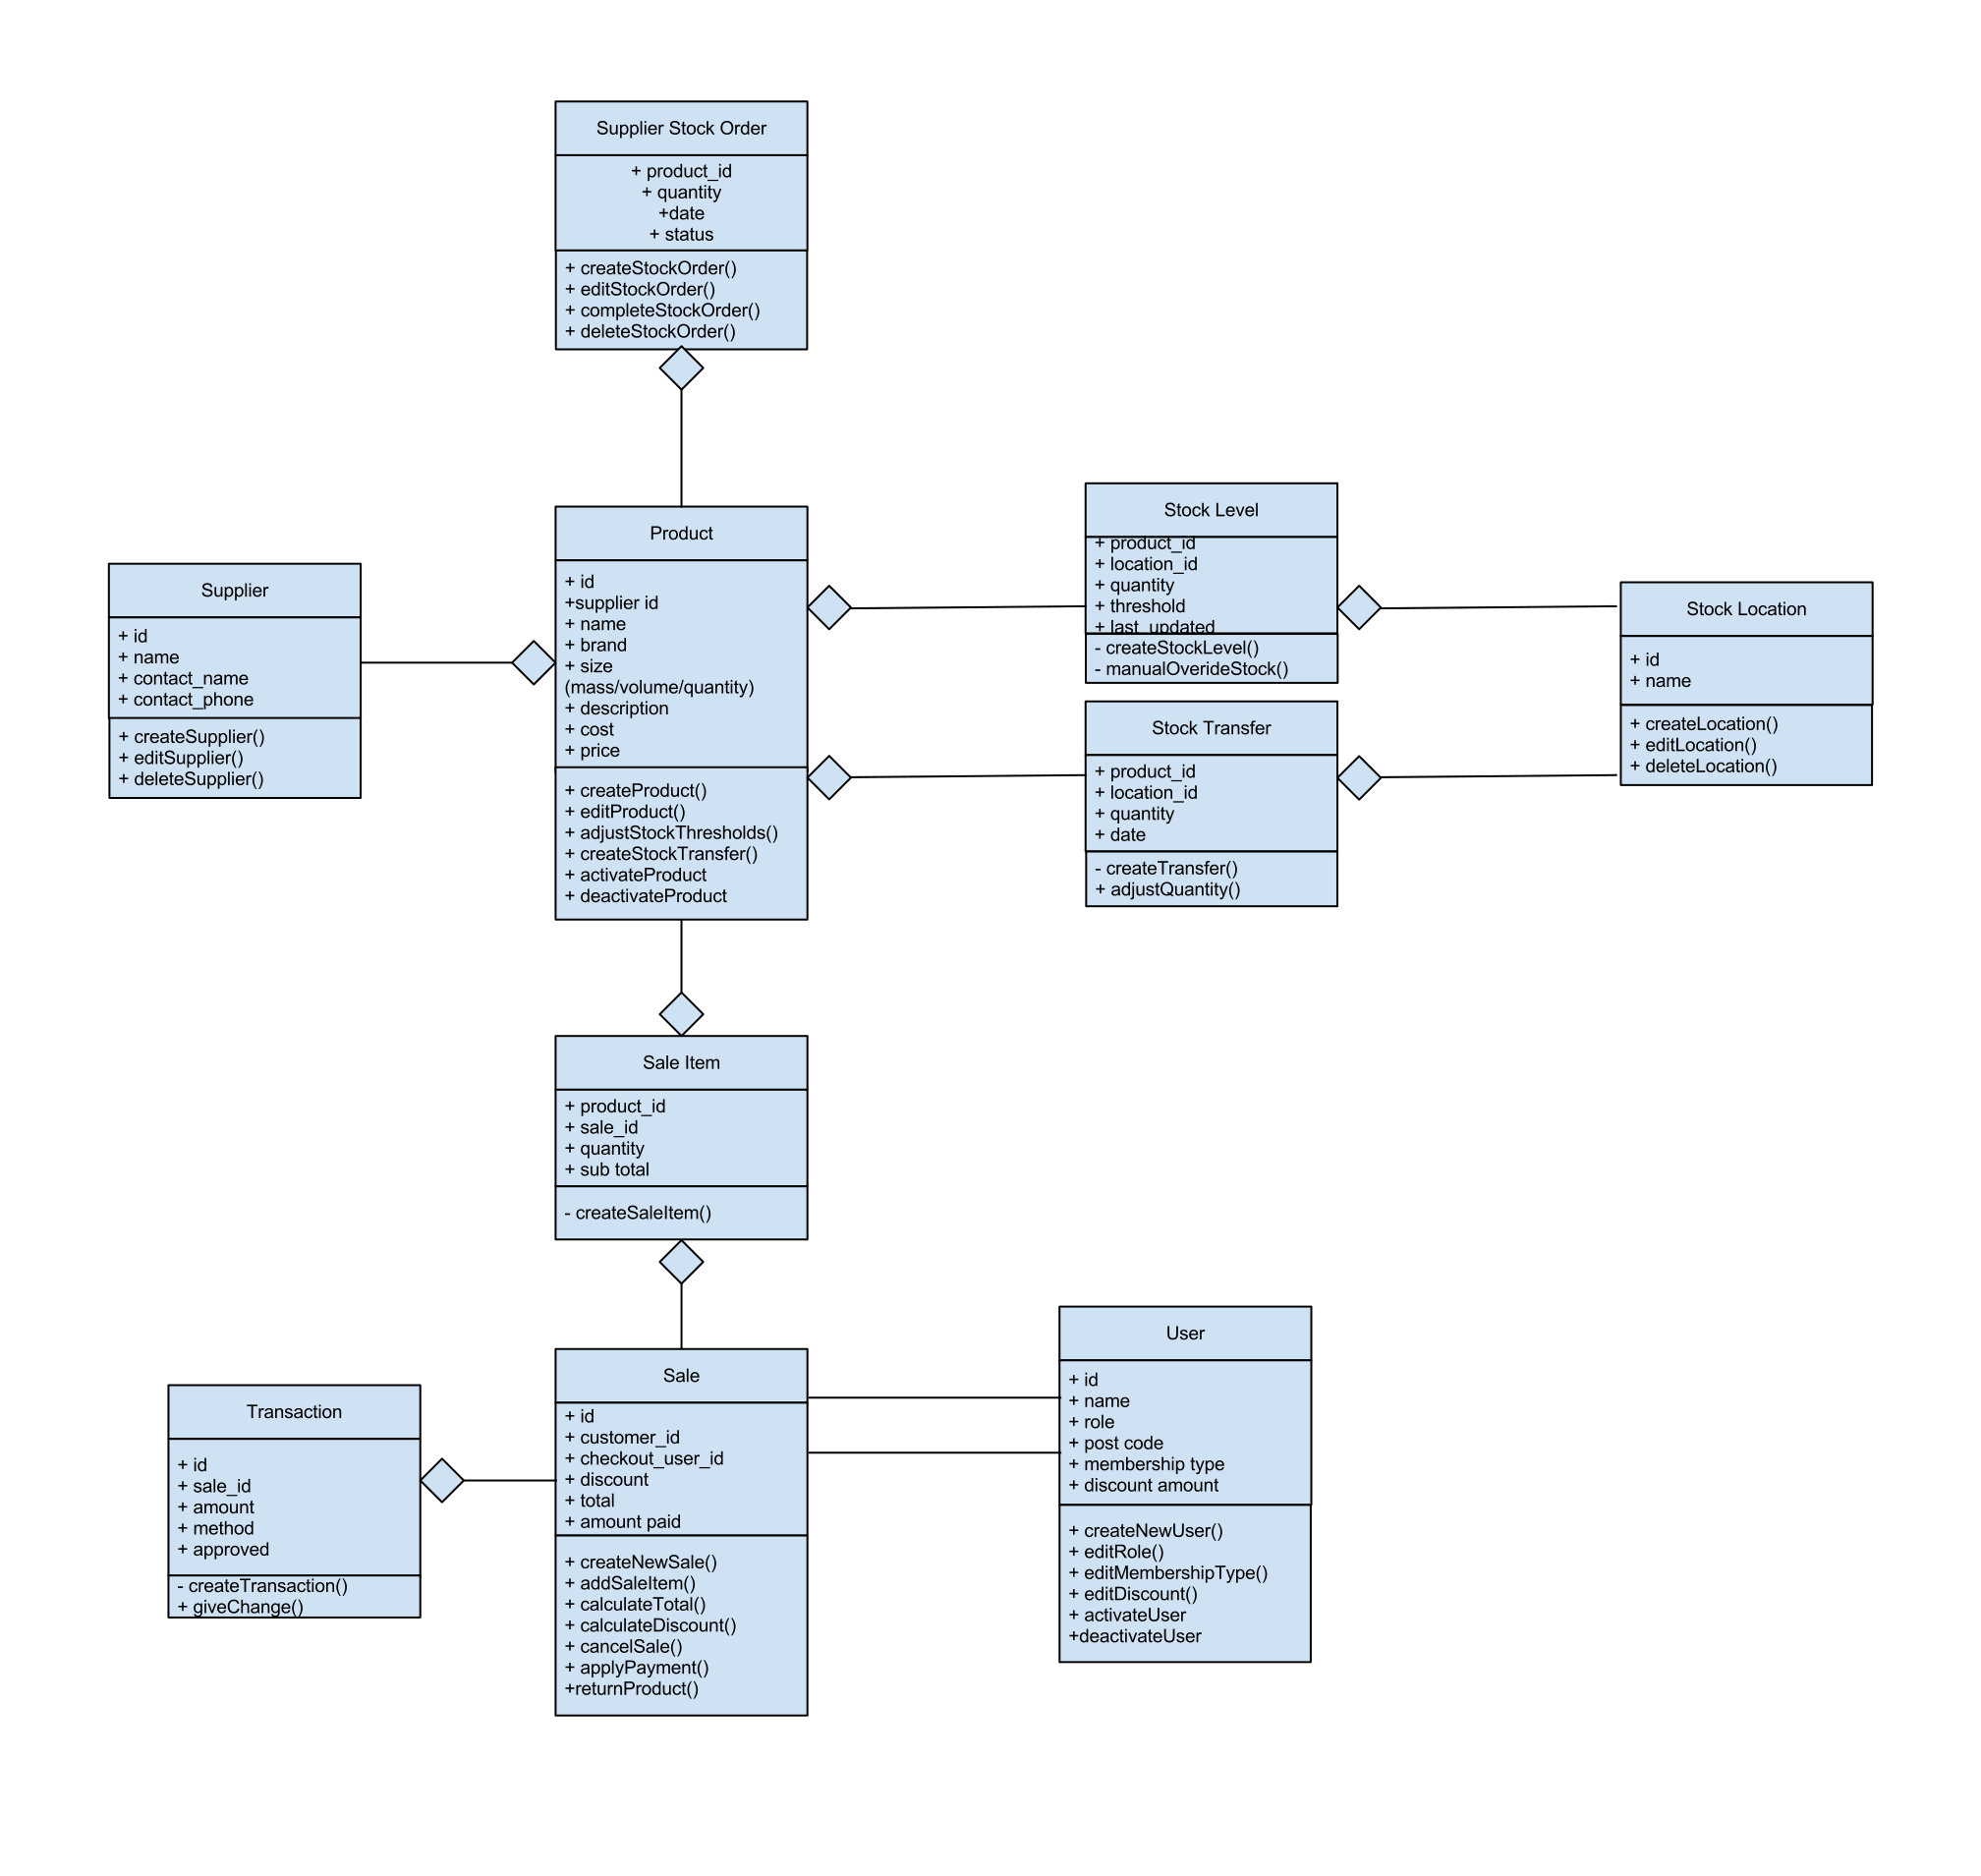
\includegraphics[scale=0.5]{Class diagram.svg}
	\caption{Standard ARM instruction encoding pattern}
\end{figure}

\pagebreak
\section{EventB to Class explanation}
All our invariants, which took one of our sets defined in the contexts and provided another set, were converted into attributes within the classes. Additional attributes in the classes were added for metadata; these mainly just consisted of description and name attributes. 

\subsection{NewORder, EditOrder, UpdateOrderToDelivering, UpdateOrderToComplete, CompleteOrder, CancelOrder}

Our event-b refinement which dealt with the ordering of products to suppliers was decomposed into a variety of classes. The main class was the 'supplier stock order' which dealt with all the attributes related to the stock orders, while the class methods were of direct correlation to the events. The attributes we extracted from the invariants were product_id, quantity, status and date. The two key invarients were \("orders ∈ activeProducts ⇸ ℕ1" and "orderStatus ∈ activeProducts ⇸ ORDER_STATUS"; \) the first shows how an order involved a product and a quantity, the second showed how orders had a status. The data attribute was simply added as metadata to provide ease of use sorting for the end-user. The events that involved ordering were converted to methods with a one to one correlation, although the events which dealt with updating the status and editing the order were merged into one method called update order. Cancel and delete were equivielant.

\subsection{NewProduct, UpdateProduct, ActivateProduct, DeactivateProduct, AutoMoveStockToFloor, AutoMoveStockToBackroom, SetProductMaxThreshol, SetProductThreshold, MoveStockToBackroom, MoveStockToFloor}

The initial refinements which dealt with the generalisation of products was decomposed into both the invariants which defined attributes and the methods. The product class was generated - as stated in previous sections all attributes were either had a direct relation with the event-b model, or were added as metadata in our class to provide the ease of use for the client. The events; NewProduct, UpdateProduct, ActivateProduct, DeactivateProduct, were added as methods to the class. The only change was the renaming of update to edit. Additionally a few events which were directly related to stock levels and products were added as methods to the products. This included creating a stock transfer and adjusting the thresholds. Overall this correlated directly to our event-b representation of products, with a large number of methods that were wrappers for calling another method on one of its relations.


\subsection{SetProductLevel, RemoveStock, AddStock}

The Stocklevel class mainly came about from the invariants in our event-b model which were used to show the relation between the products and stock_locations. This invariant "productlevels ∈ products →(STOCK_LOCATION → ℕ)"  was the cause for the main attribute of the class, although additional attributes were added as a form of metadata. The main events which were ported to this class as methods were the events to do with directly altering product levels, ie settproductlevel, removestock and addstock. These are all merged into a private manual override method.

\subsection{NewMember, SetMemberDiscount, RemoveCreditToMemberAccount, addCredit to MemberAccount, DeactivateMembers, ActivateMembers,NewUser, EditUserPriveleges}

Within our event-b model we had two sets for both the members and users, as it provided the easiest form of modelling our solution at the time. However when we begun to work on our class diagram we could see that they were both virtually the same and any attributes that were only in one of them could be consider as metadata for the other. Hence we decided to merge both the member and user in the class diagram to the user class, all the attributes either came from the invarients which linked to either user or members to certains sets. The NewMember and NewUser were converted into the createUserMethod of our class, the editrole method had a direct corolation to to the edituserpriveleges, but the only change that will actually occur in the method is that there is now an option for the role of basicmember. The edit membertype and editdiscount methods were used to replace the setmemberdiscount, removecredit and addcredit events in our model. 

Overall even though we merged user and meber it still had a direct relation to the event=b model that we had created. 


\subsection{NewCart, CalculateTotalCart , AddProductToCart, CancelCheckOut}

Our event-b model had the notion of carts and recipts, during the design process we decided that the best way to convert it into class diagram was to split these intow two objects one of which was a the sale class, and the other saleitemclass. The newcart event was added to the sale  calss as a method named create new sale, similartly add producttocart was replaced by a method with the name add sale item, and finally calculatetotalcart, was just simply shortened and added as a method name calculate total. All invariants involving sales were also added as attributes, although a few additional attributes were added as a form of metadata. CancelCheckout from our event-b model was also renamed as a mehtod of sale and it was renamed to cancel sale but still provided the same functionality and consistency. Additionally the returnProduct  event was added to this class as a method to ensure that integrity was kept between our design and our event b model.

\subsection{PayForCartCash, PayForCartOtherPaymentType, PayCash}

The event-b refinement which involved, paying for a cart were modeled into the  classes through the uses of the payment classes. The way in which multiple payments could be used in the event-b model was replicated in the class diagram through the way in which sales could have multiple payments. All the events for paying were basically converted to the one method, which was create payment the only difference is that the the create payment method would be called with different parameters. The attributes stored in the class are basically only used as metadata, and provide no extra validity to the event-b model but just focused on adding functionality for the end user. The GiveChangeCash event from our model was directly changed to a method givechange in of the transaction class and allows for payments to pay with larger amounts and recieve change.

\subsection{ProceedToPayment, ProceedToCheckout}

These events from our event-b model are not directly modelled in our class diagram as they do not specifically involve the persistant data, and hence would be used in the transaction controller. 

\pagebreak
\section{System Architecture}

The architecture of our final solution will rely heavily on the use of common design patterns such as MVC. Since it is so widely used in industry, there are many publications to date describing the design and use of MVC quite extensively which do not need to be repeated here. As such, this report will assume you have a working knowledge of MVC and instead focus on how it relates to our design.

During implementation, it determined that translating Stock\_Control and its refinements directly into an instance of MVC would be unfeasible. Its size and complexity would most likely cause several issues in maintaining consistency and correctness without invariants, guards and the various other tools offered by EventB. As a result, the machine will be split into several instances of MVC.

For example, the Product class in the class diagram is actually an instance of MVC with it’s own model, view and controller. Similarly, almost all classes in that diagrams are actually MVC instances that have been illustrated as a single class for the sake of simplicity.

\subsection{View}

A view’s role is to represent state of machine in a meaningful way to the user. It also needs to have a way of allowing the user to trigger any of the events in a machine, provided all the guards are met.

In our system, most of the views will be rendered in a browser, primarily due to ease of deployment.

For example, the view for a product will show its id, cost, price as well as some decorative details like name, brand, size, description etc. It will probably render these in a web page with nicely laid out labels in when the user is viewing a product, and with textboxes and spinners when they want to edit. There will be buttons to add new products, de/reactivate products and to start all other relevant events. 

\subsection{Controller}

A controller is what responds to the requests created by the views and actually performs the required actions. Logically, most of the methods corresponding to events will go in controller classes. 

Continuing the above example, if a user presses the button to deactivate a product, the product controller will mark that product as ‘inactive’, just as the deactivateProduct event would.

\subsection{Model}

A model’s role, in relation to an EventB machine, is fairly straightforward. It needs to persistently store a variable from a machine, and provide methods for controllers to use this data. 
While some variables that were very tightly related in the machine were stored in the same model, but in general, it boiled down to about one model per variable. Not only did this allow each variable to be stored in a way that suited it best, but since a controller usually only needs to deal with one EventB variable at a time, this allowed those interfaces to be clean and uncluttered. 

So, the Product model essentially looks after the products and activeProducts variable from the eventB machine. It normalizes and stores them (along with all the details required) in an SQL database. It also builds queries and retrieves data required by controllers to function and views to display. 
\pagebreak
\section{Sequence Diagrams and Use Cases}

\pagebreak
\section{Design Discussion}

\pagebreak

\section{Appendix}

\appendix


\end{document}

